%
% Acta Acustica united with Acustica -- Instructions for Authors, 2017-03-01
%
\documentclass[twocolumn]{article}

%%%%%%%%%%%%%%%%%%%%%%%%%%%%%%%%%%%%%%%%%%%%%%%
%% Comment / uncomment for one or two column(s) fomat
%\documentclass{article}

\usepackage[modulo,switch]{lineno}
\modulolinenumbers[1]
%%%%%%%%%%%%%%%%%%%%%%%%%%%%%%%%%%%%%%%%%%%%%%%
%% Comment / uncomment for showing line numbers
 \linenumbers

\usepackage[utf8]{inputenc}
\usepackage{amsmath}
\usepackage{amssymb}
\usepackage{float}
\usepackage{graphicx}

\makeatletter\@ifundefined{date}{}{\date{}}
\makeatother

%\markright{\hfill Kergomard {\em et al.}, p.\ }
\pagestyle{myheadings}

\paperheight297mm \paperwidth210mm
\textwidth170mm  \textheight245mm  \oddsidemargin 20mm
\evensidemargin\oddsidemargin \hoffset-22.4mm \voffset-28.4mm
\topmargin0pt \headheight20mm \headsep4mm \topskip0mm
\footskip17.5mm \columnsep7mm \arraycolsep2pt \parindent10pt
\renewcommand{\abstractname}{Introduction}

\begin{document}

\title{TTT4180 Technical Acoustics - Assignment 7}

\author{Nicholas Bresina, Department of Electronic Systems, NTNU Trondheim, Norway \\
nicholdb@stud.ntnu.no}

\maketitle\thispagestyle{empty}

\begin{abstract}
This assignment in the Technical Acoustics course (TTT4180) revolves around
the transmission-line matrix (TLM) simulation technique used for acoustic waves
and studying a variety of acoustic wave propagation scenarios by simulation.
The report is split into two parts, where the first part provides a brief
description of methods used for an own implementation of TLM simulation in Python.
After, some results are presented and discussed, which were generated from said
implementation.
The second part contains further analyisis of sound pressure
with respect to distance, surface reflections, and the effect of a noise screen
on the sound pressure level.
Instead of using the own implementation, this part uses a given Matlab implementation
called TLMfig.
Lastly, the report gives a brief outlook with a discussion of difficulties
encountered during this assignment and final conclusions.
% Possibly add difficulties and gained knowledge
\end{abstract}


\section{Python Implementation}
To analyze the propagation of a wave in a pipe a 2D TLM implementation was needed.
Python was chosen, as it provides all of the necessary features in libraries such
as Numpy for arrays and linear algebra and Matplotlib for plotting the results.

\subsection{Methods}
The implementation is strongly based on the article provided with the assignment
that describes TLM \cite{KagawaTLM}.
Nevertheless the most significant parts will be described in this section.

The main idea is to replace the continuous space with a mesh of so-called nodes,
as shown in Fig. \ref{fig_tlm_mesh}.

\begin{figure}[H]
    \centering
    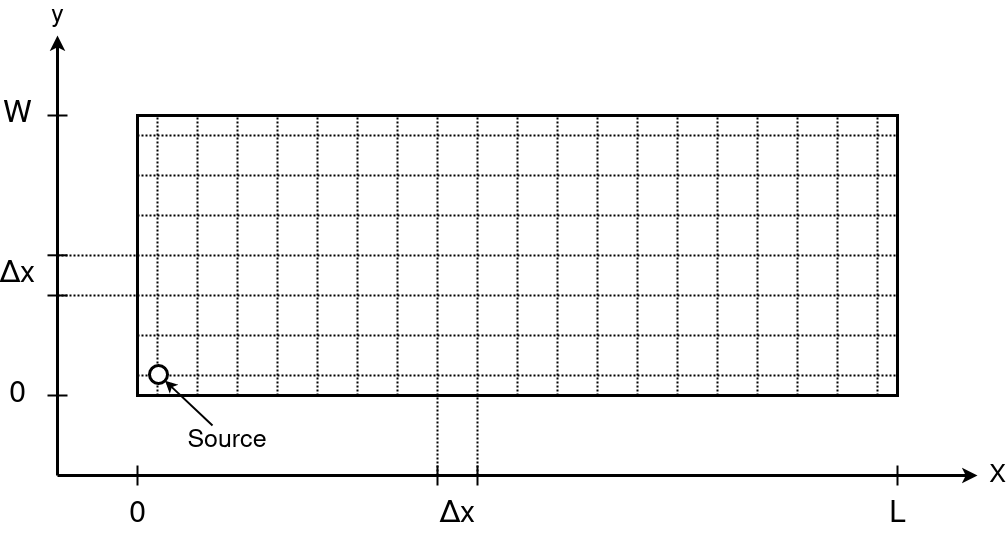
\includegraphics[width=75mm]{./Images/tlm_pipe.png}
    \caption{Example for TLM mesh placed on a pipe with dimensions L$\times$W}
    \label{fig_tlm_mesh}
\end{figure}


\subsection{Results}

\subsection{Discussion}

\section{TLMFig}
\subsection{Results}

\subsection{Discussion}

\section{Conclusion}

\section{References}

\small
\bibliographystyle{plain}
\bibliography{references.bib}

\end{document}
